\documentclass[12pt]{exam}
%\documentclass[12pt]{article}
\usepackage[letterpaper, margin=0.75in]{geometry}
\usepackage{graphicx}
\usepackage{enumitem}
\usepackage{booktabs}
\usepackage{amsmath}
\usepackage{tabularx}
\usepackage{color}

\begin{document}
\footer{}{Page \thepage\ of \numpages}{}

\begin{flushright}
\makebox[0.5\textwidth]{\large Name:\enspace\hrulefill}
\vspace{0.2in}

\makebox[0.5\textwidth]{\large Date:\enspace\hrulefill}
\end{flushright}

\begin{center}

\includegraphics[width=10cm]{../images/logo.png}
\end{center}

\begin{center}
\noindent{\LARGE Conceptual Physics \\ Class 9 Questions \\ April 6th, 2018 \\}
\end{center}

\vspace{0.2in}

The following might be useful for today's class questions:
\begin{center}
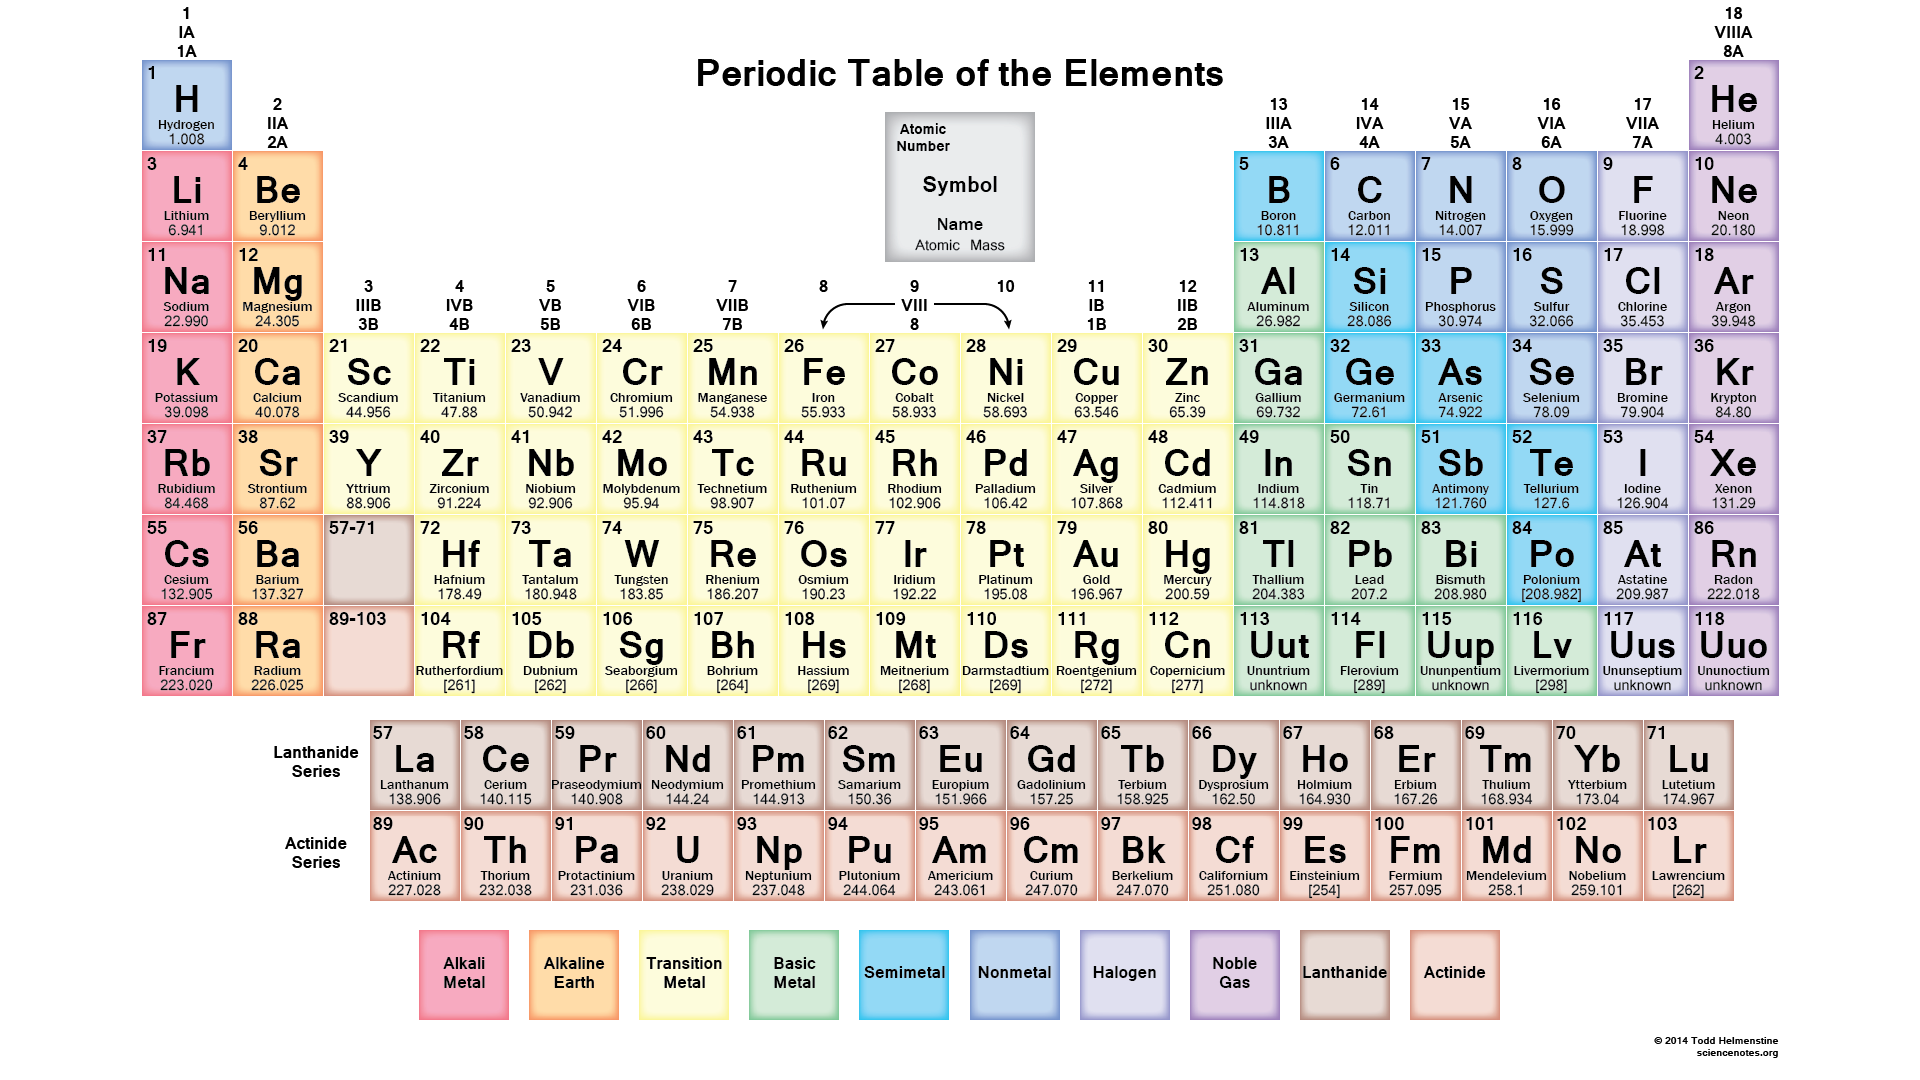
\includegraphics[width=\textwidth]{../images/periodicTable.png}
\end{center}


\clearpage

\begin{questions}
	\question The following is a wave of light:
	\begin{center}
	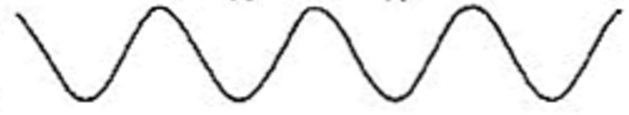
\includegraphics[width=4in]{../images/wavelength.png}
	\end{center}
	\begin{parts}
		\part Draw the light-wave \textit{red-shifted}.
		\vspace{1in}
		
		\begin{itemize}
			\item What happens to the frequency? (Increase, decrease, stay the same):
				\vspace{0.3in}
			\item What happens to the wavelength? (Increase, decrease, stay the same):
				\vspace{0.3in}
			\item What happens to the energy? (Increase, decrease, stay the same):
				\vspace{0.3in}
			\item What happens to the intensity? (Increase, decrease, stay the same):
				\vspace{0.3in}
		\end{itemize}
		
		\part Draw the light-wave \textit{blue-shifted}
		\vspace{1in}
		
		\begin{itemize}
			\item What happens to the frequency? (Increase, decrease, stay the same):
				\vspace{0.3in}
			\item What happens to the wavelength? (Increase, decrease, stay the same):
				\vspace{0.3in}
			\item What happens to the energy? (Increase, decrease, stay the same):
				\vspace{0.3in}
			\item What happens to the intensity? (Increase, decrease, stay the same):
				\vspace{0.3in}
		\end{itemize}
	\end{parts}
	
	\clearpage
	\question In the Doppler effect, light is red-shifted or blue-shifted depending on whether objects are moving away from each other or closer together.
		\begin{parts}
			\part When two objects come together, light is \textit{blue-shifted} between them. What happens to:
				\begin{enumerate}
					\item The wavelength of the light? (Increase, decrease, stay the same):
						\vspace{0.2in}
					\item The frequency of the light? (Increase, decrease, stay the same):
						\vspace{0.2in}
					\item The energy of the light? (Increase, decrease, stay the same):
						\vspace{0.2in}
					\item The intensity of the light? (Increase, decrease, stay the same):
						\vspace{0.2in}
				\end{enumerate}
			\part When two objects move away from each other, light is \textit{red-shifted} between them. What happens to:
				\begin{enumerate}
					\item The wavelength of the light? (Increase, decrease, stay the same):
						\vspace{0.2in}
					\item The frequency of the light? (Increase, decrease, stay the same):
						\vspace{0.2in}
					\item The energy of the light? (Increase, decrease, stay the same):
						\vspace{0.2in}
					\item The intensity of the light? (Increase, decrease, stay the same):
						\vspace{0.2in}
				\end{enumerate}
		\end{parts}
	
	\question The following diagram represents the EM spectrum of light.
	\begin{center}
		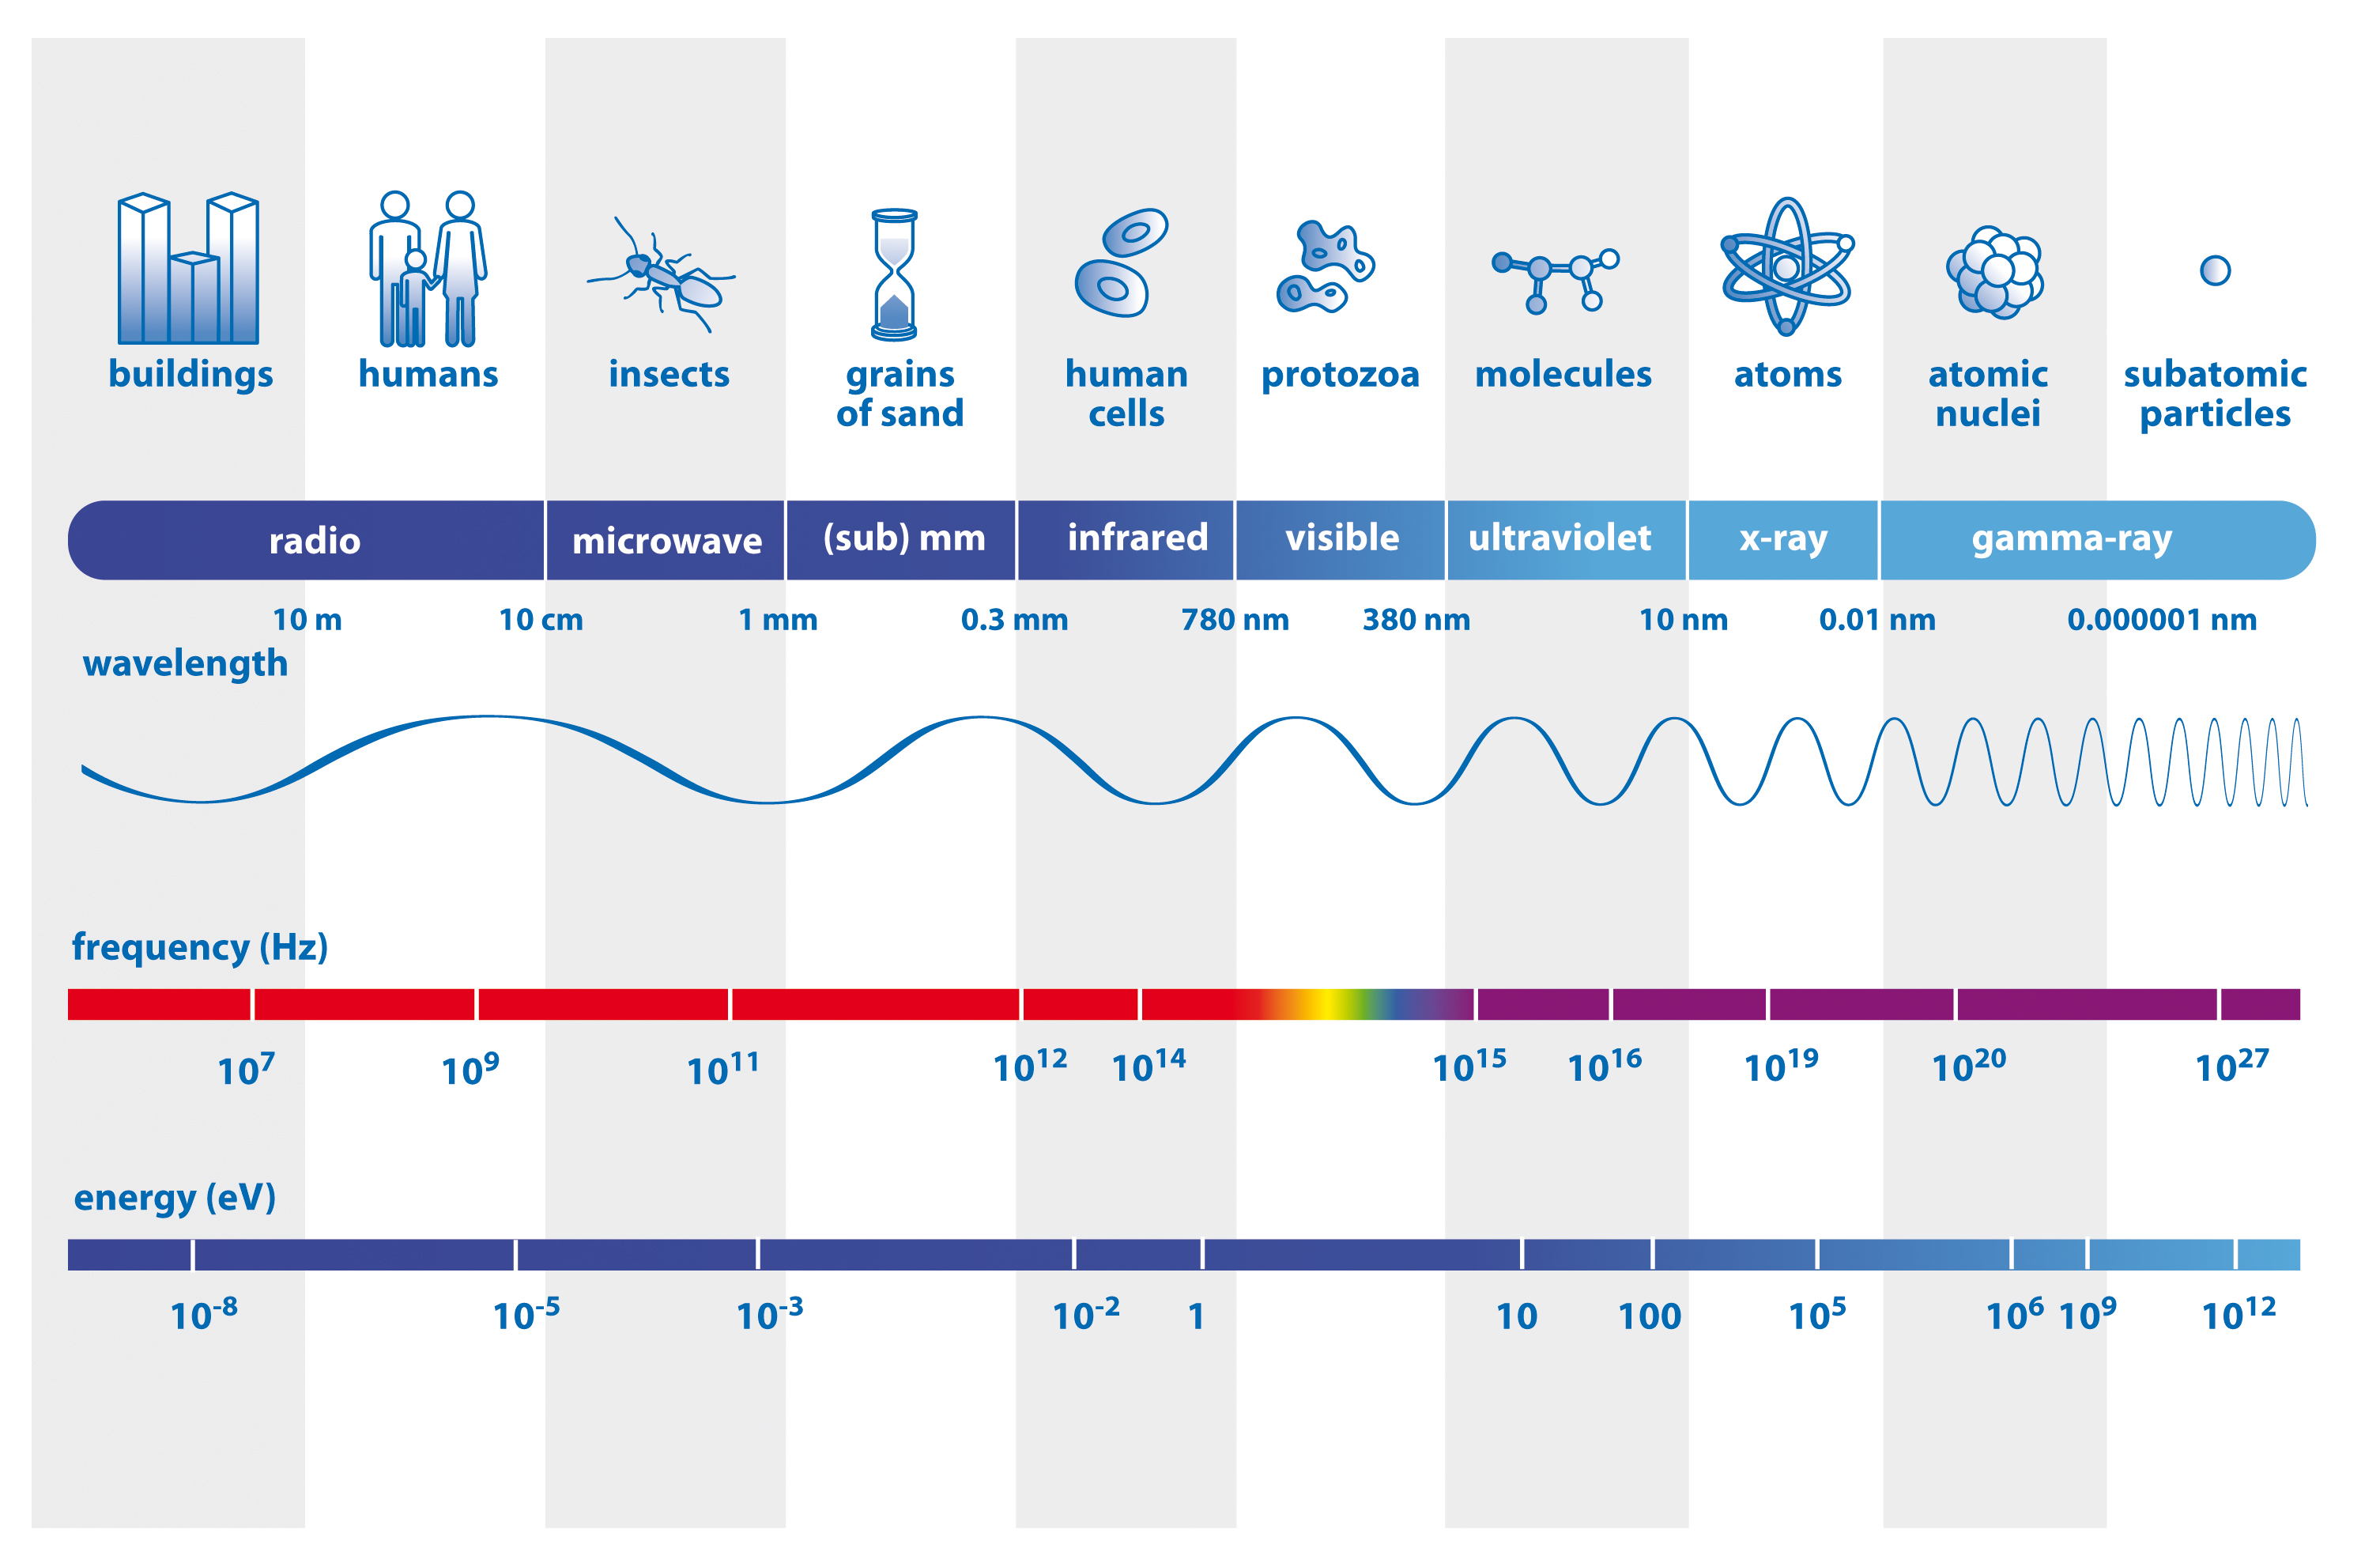
\includegraphics[width=0.5\textwidth]{../images/emSpectrum.jpg}
	\end{center}		
	
	\begin{parts}	
		\part Order the following photons in terms of \textit{increasing energy:} x-rays, microwaves, infrared, visible light
			\vspace{0.1in}
		\part Which has the greater \textit{wavelength}: Radiowaves or infrared?
			\vspace{0.1in}
		\part Which has the greater \textit{frequency}: Visible light or gammarays?
			\vspace{0.1in}
	\end{parts}
	
\clearpage
\question When light is reflected from a mirror, perhaps only 80\% of the energy comes back. The rest is converted to heat. One could try to explain this in two different ways: (1) 80\% of the photons are reflected, or (2) all the photons are reflected, but each loses 20\% of its energy. Based on your everyday knowledge about mirrors, how can you tell which interpretation is correct?

From \textit{Light and Matter}, Chapter 34 Question 3	
\vspace{1in}	
	
	\question Two cars are driving in opposite directions on a road, by a pedestrian.
	\begin{center}
	\input{../images/carsPerson.pdf_tex}
	\end{center}
	
	\begin{parts}
		\part To the pedestrian on the road, the lights from car A appear
			\begin{enumerate}
				\item Red-shifted
				\item Blue-shifted
				\item Unchanged
			\end{enumerate}
		\part To the pedestrian on the road, the lights from car B appear
			\begin{enumerate}
				\item Red-shifted
				\item Blue-shifted
				\item Unchanged
			\end{enumerate}
		\part To car A, the lights from car B appear:
			\begin{enumerate}
				\item Red-shifted
				\item Blue-shifted
				\item Unchanged
			\end{enumerate}
		\part To car B, the lights from car A appear:
			\begin{enumerate}
				\item Red-shifted
				\item Blue-shifted
				\item Unchanged
			\end{enumerate}
		\part Compare and contrast the light from car A, as it appears to car B and the pedestrian.
		\vspace{0.5in}
		\part Compare and contrast the light form car B, as it appears to car A and the pedestrian.
		\vspace{0.5in}
	\end{parts}
	
	\clearpage
	\question You are standing by the side of the road, and West of you is a stationary car with its lights on, labelled as (1) in the image below. The car then begins to move, and accelerates East. Part (2) shows the car some time later, moving East and still accelerating. Part (3) shows the car at its highest velocity, which it maintains as it moves past you to part (4). The car then begins to slow down, and so has the same velocity in part (5) as in part (2), and then comes to a complete stop again at point (6). The image bellow illustrates this, where the car's velocity is indicated by the arrows. Use this to answer the following questions.
\vspace{0.1in}
\begin{center}
\input{../images/finalDoppler.pdf_tex}
\end{center}
\vspace{0.1in}

\begin{parts}
	\part At which point(s) if any do the car's lights appear red-shifted to you?
		\vspace{1in}
	\part At which point(s) if any do the car's lights appear blue-shifted to you?
		\vspace{1in}
	\part At which point(s) if any are the car's light neither red nor blue-shifted?
		\vspace{1in}
\end{parts}

	\clearpage
	\question Carbon comes in 3 main isotopes, carbon-12, carbon-13 and carbon-14.
		\begin{parts}
			\item How many protons are in a carbon-12 atom?
				\vspace{0.3in}
			\item How many protons are in a carbon-13 atom?
				\vspace{0.3in}
			\item How many protons are in a carbon-14 atom?
				\vspace{0.3in}
			\item How many neutrons are in a carbon-12 atom?
				\vspace{0.3in}
			\item How many neutrons are in a carbon-13 atom?
				\vspace{0.3in}
			\item How many neutrons are in a carbon-14 atom?
				\vspace{0.3in}
		\end{parts}
	
	\question The weak nuclear force mediates a form of nuclear decay, where a neutron turns into a proton and in the process emits an electron and an \textit{anti-}neutrino. This is called \textit{beta decay}:
	\begin{eqnarray}
	n \rightarrow p^+ + e^- + \bar{\nu} \nonumber
	\end{eqnarray}
	\begin{parts}
		\part What is the total electrical charge on the left hand side of this reaction (just the neutron?)
			\vspace{0.2in}
		\part What is the total electrical charge on the right hand side of this reaction (proton, electron, anti-neutrino) if the anti-neutrino has no charge?
			\vspace{0.2in}
		\part A comparable decay mediated by the weak force is one where the proton decays. However, in this process a proton decays to a neutron by forming a \textit{positron}, a particle of anti-matter which is the exact opposite of the electron, and a neutrino
		\begin{eqnarray}
		p^+ \rightarrow n + e^+ + \nu \nonumber
		\end{eqnarray}
		What is the total electrical charge on the left hand side of this reaction (just the proton)?
			\vspace{0.2in}
		\part What is the total electrical charge on the right hand side of this reaction (neutron, positron, neutrino)?
			\vspace{0.2in}
		\part From the above two reactions, you should notice that the amount of charge is the same on both sides. This is because electrical charge is a conserved quantity in nature (think back to Noether's theorem, there's a symmetry in the electric field that makes this true). Knowing this, explain whether or not the following decay is possible:
		\begin{eqnarray}
		p^+ \rightarrow n + e^- + \nu \nonumber
		\end{eqnarray}
		\vspace{0.2in}
		
		\part \textit{Electron capture} is the process by which an electron an proton come together to form a neutron (releasing a neutrino in the process). Using the idea of conservation of charge, explain why this is possible:
		\begin{eqnarray}
		p^+ +e^- \rightarrow n + \nu \nonumber
		\end{eqnarray}
		\vspace{0.2in}
	\end{parts}
	
	\question The following isotopes undergo either \textit{beta decay} or \textit{electron capture} (described in the previous question). What do they turn into?
	\begin{parts}
		\part Cobalt-57 undergoes electron capture
			\vspace{0.2in}
		\part Carbon-14 undergoes beta decay
			\vspace{0.2in}
		\part Aluminum-26 undergoes electron capture
			\vspace{0.2in}
		\part Cesium-137 undergoes beta decay
			\vspace{0.2in}
		\part Sodium-22 undergoes electron capture
			\vspace{0.2in}
		\part Beryllium-7 undergoes electron capture
			\vspace{0.2in}
		\part Iron-55 undergoes electron capture
			\vspace{0.2in}
	\end{parts}
	
	\question When an antielectron and an electron come together, they annihilate causing a gamma ray to be released:
	\begin{eqnarray}
	e^- + e^+ \rightarrow \gamma \nonumber
	\end{eqnarray}
	Is charged conserved in this reaction?
	\vspace{0.3in}
	
	\clearpage
	\question In very heavy elements (with lots of neutrons and protons in a nucleus), there are many ways in which the nucleus can be arranged.
	\begin{center}
	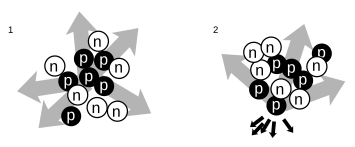
\includegraphics[width=0.4\textwidth]{../images/nucleotide_arrangements.png}
\end{center}	
The image is taken from \textit{Light and Matter}, Chapter 26.
\begin{parts}
	\part What are the two dominant forces acting on the protons in the two figures?
		\vspace{1in}
	\part Very heavy elements tend to be \textit{neutron rich}, meaning that they have far more neutrons than protons. Using the above figure and the forces you listed in part (a), explain why.
		\vspace{0.2in}
\end{parts}
	
	\clearpage
	\question \textit{Nuclear fusion} is the process by which atomic nuclei come together to create heavier elements.
	
	\textit{Nuclear fission} is the process by which atomic nuclei break apart to create lighter elements.
	
	The amount of energy released is related to the \textit{binding energy} of the atom: It is the amount of energy needed to disassemble the nucleus into free protons and neutrons.
	\begin{center}
		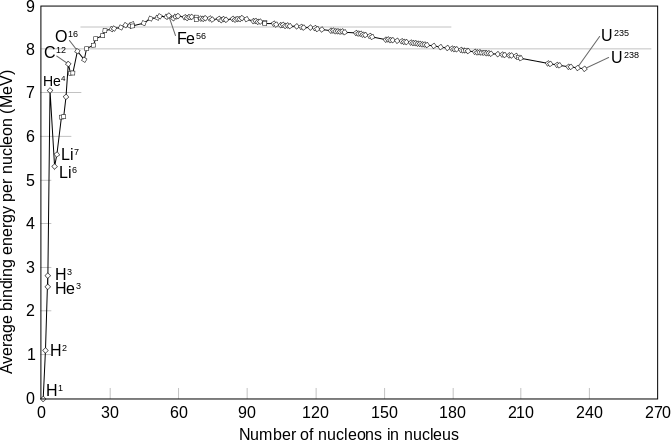
\includegraphics[width=0.8\textwidth]{../images/bindingEnergies.png}
	\end{center}
	
	\begin{parts}
		\item When hydrogen-1 ($^1$H) comes together with free neutrons to create helium-3 ($^3$He), would the process release or require energy?
			\vspace{0.5in}
		\item If helium-4 ($^4$He) broke into hydrogen-2 ($^2$H), would the process release or require energy?
			\vspace{0.5in}
		\item Why does the sun release energy by fusing lighter elements (hydrogen, helium) whereas nuclear reactors release energy by breaking apart heavier elements (uranium, plutonium)?
			\vspace{0.5in}
		\item Following this argument, why is iron-56 ($^{56}$Fe) the most stable nucleus?
			\vspace{0.5in}
	\end{parts}
\end{questions}

\end{document}
